\documentclass{article}

\usepackage{tikz}

\usetikzlibrary{external}
\tikzexternalize


\begin{document}


% Perceptron
\tikzsetnextfilename{perceptron}
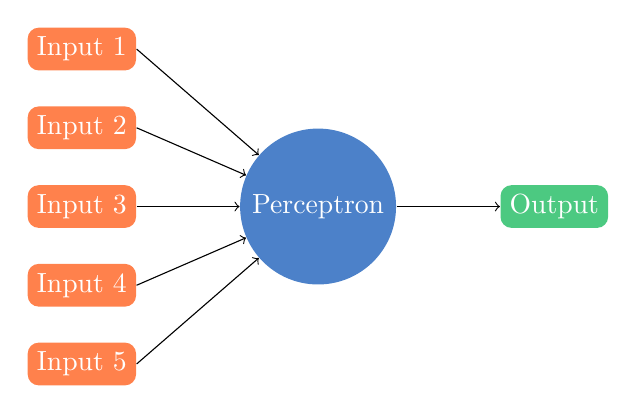
\begin{tikzpicture}

\tikzstyle perc=[circle, fill=blue!70!green, fill opacity=.7, text=white, text opacity=1]
\tikzstyle input=[rounded corners, fill=red!70!yellow, opacity=.7, text=white, text opacity=1]
\tikzstyle output=[rounded corners, fill=green!70!blue, opacity=.7, text=white, text opacity=1]

\node (p) [perc] at (0,0) {Perceptron};
\node (i1) [input] at (-3,2)  {Input 1};
\node (i2) [input] at (-3,1)  {Input 2};
\node (i3) [input] at (-3,0)  {Input 3};
\node (i4) [input] at (-3,-1) {Input 4};
\node (i5) [input] at (-3,-2) {Input 5};
\node (o) [output] at (3,0) {Output};

\draw [->] (i1.east) -- (p);
\draw [->] (i2.east) -- (p);
\draw [->] (i3.east) -- (p);
\draw [->] (i4.east) -- (p);
\draw [->] (i5.east) -- (p);
\draw [->] (p.east) -- (o);

\end{tikzpicture}


% Neural Netowrk 1 
\tikzsetnextfilename{neural-network-1}
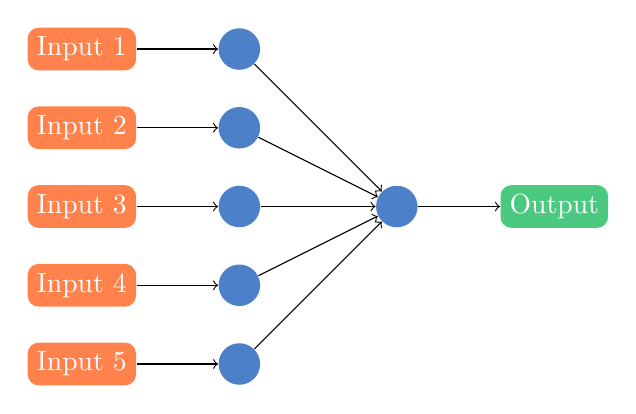
\begin{tikzpicture}

\tikzstyle perc=[circle, minimum size=15pt, fill=blue!70!green, fill opacity=.7, text=white, text opacity=1]
\tikzstyle input=[rounded corners, fill=red!70!yellow, opacity=.7, text=white, text opacity=1]
\tikzstyle output=[rounded corners, fill=green!70!blue, opacity=.7, text=white, text opacity=1]

\node (p) [perc] at (1,0) {};

\node (p1) [perc] at (-1,2)  {};
\node (p2) [perc] at (-1,1)  {};
\node (p3) [perc] at (-1,0)  {};
\node (p4) [perc] at (-1,-1) {};
\node (p5) [perc] at (-1,-2) {};

\node (i1) [input] at (-3,2)  {Input 1};
\node (i2) [input] at (-3,1)  {Input 2};
\node (i3) [input] at (-3,0)  {Input 3};
\node (i4) [input] at (-3,-1) {Input 4};
\node (i5) [input] at (-3,-2) {Input 5};
\node (o) [output] at (3,0) {Output};

\foreach \i in {1,...,5}
{
\draw [->] (i\i.east) -- (p\i);
\draw [->] (p\i) -- (p);
}

\draw [->] (p.east) -- (o);

\end{tikzpicture}



% Neural Network 2 
\tikzsetnextfilename{neural-network-2}
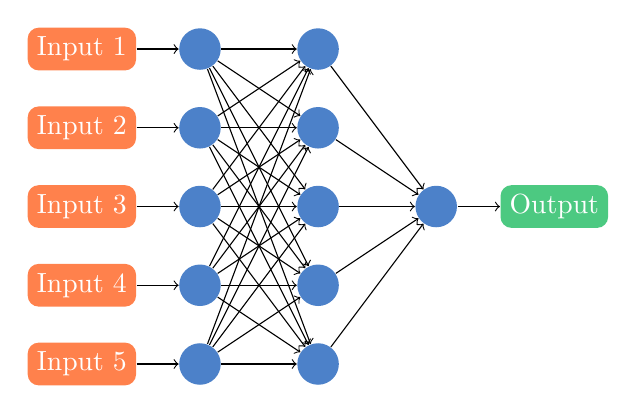
\begin{tikzpicture}

\tikzstyle perc=[circle, minimum size=15pt, fill=blue!70!green, fill opacity=.7, text=white, text opacity=1]
\tikzstyle input=[rounded corners, fill=red!70!yellow, opacity=.7, text=white, text opacity=1]
\tikzstyle output=[rounded corners, fill=green!70!blue, opacity=.7, text=white, text opacity=1]

\node (p) [perc] at (1.5,0) {};

\node (p1) [perc] at (-1.5,2)  {};
\node (p2) [perc] at (-1.5,1)  {};
\node (p3) [perc] at (-1.5,0)  {};
\node (p4) [perc] at (-1.5,-1) {};
\node (p5) [perc] at (-1.5,-2) {};

\node (p11) [perc] at (0,2)  {};
\node (p12) [perc] at (0,1)  {};
\node (p13) [perc] at (0,0)  {};
\node (p14) [perc] at (0,-1) {};
\node (p15) [perc] at (0,-2) {};

\node (i1) [input] at (-3,2)  {Input 1};
\node (i2) [input] at (-3,1)  {Input 2};
\node (i3) [input] at (-3,0)  {Input 3};
\node (i4) [input] at (-3,-1) {Input 4};
\node (i5) [input] at (-3,-2) {Input 5};
\node (o) [output] at (3,0) {Output};

\foreach \i in {1,...,5}
{
\draw [->] (i\i.east) -- (p\i);
\draw [->] (p1\i) -- (p);
	\foreach \j in {1,...,5}
	{
	\draw [->] (p\i) -- (p1\j);
	}
}

\draw [->] (p.east) -- (o);

\end{tikzpicture}

\end{document}

